% use \pts{} to indicate the number of points

% Define numbers here (everything calculated from these values)
\newcommand{\qFs}{1000}
\newcommand{\qPer}{50}
\newcommand{\qPh}{16}

\clearpage
The following graph contains samples of a signal. The sampling rate was \textbf{\qFs\, Hz}.

\begin{center} % Insert a plot
  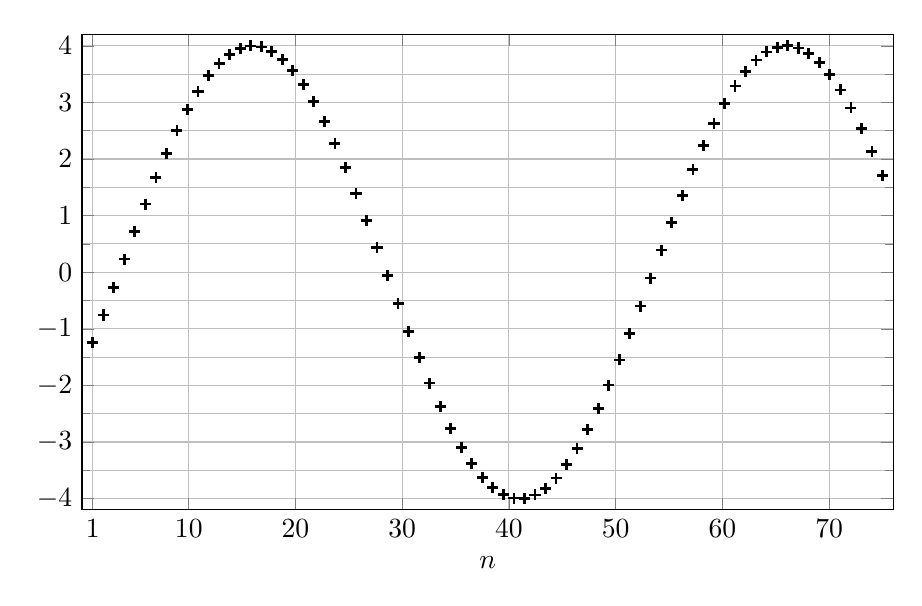
\begin{tikzpicture}
    \begin{axis}[
      width=.98\textwidth,
      height=3in,
      axis lines=box,
      xlabel=$n$,
      ylabel={},
      xmin=0,
      xmax=76,
      ymin =-4.2, ymax = 4.2,
      ytick = {-4, -3, ..., 4},
      grid=both,
      xtick = {1, 10, 20, ..., 80},
      minor tick num=1,
      ]
      \addplot[
      only marks,
      domain=1:75,
      samples=76, 
      color=black, 
      mark=+, 
      line width=1pt,
      ] 
      {4*cos(deg(2 * pi / \qPer * x - 2 * pi * \qPh / \qPer))};

    \end{axis}
  \end{tikzpicture}
\end{center}

%% Anwer:
%% : A: 4
%% : freq: 66-16 = 50 sp/period
%% : Fs / 50 = 1000 / 50 = 20 Hz
%% : phase: -2*pi * (16/50)
%% : x(t) = 4 * cos( 2*pi*20*t - 0.64 * pi)

Give an expression for $y(t)$ that represents the original continuous-time signal including \textbf{amplitude} [2 points], \textbf{frequency (Hz)} [4 points], and \textbf{phase} [4 points].

%% OK, this redefines how a question in AMC is created so that everything can be closer together. I re-redefine it back to normal at the bottom of this question.

%\def\AMCbeginQuestion#1#2{\par\noindent{\bf Question #1} #2\hspace*{1em}}
\def\AMCbeginQuestion#1#2{}
\begin{question}{03-lSineA}
  \AMCOpen{lines=1,
    dots=false,  }{\wrongchoice[W]{w}\scoring{0}\wrongchoice[P]{p}\scoring{2}\correctchoice[C]{c}\scoring{4}}
\end{question}

\begin{question}{03-lSineF}
  \AMCOpen{lines=1,
    dots=false,  }{\wrongchoice[W]{w}\scoring{0}\wrongchoice[P]{p}\scoring{2}\correctchoice[C]{c}\scoring{4}}
\end{question}
\begin{question}{03-lSinePh}
  \AMCOpen{lines=1,
    dots=false,  }{\wrongchoice[W]{w}\scoring{0}\wrongchoice[P]{p}\scoring{2}\correctchoice[C]{c}\scoring{4}}
\end{question}
\def\AMCbeginQuestion#1#2{\par\noindent{\bf Question #1} #2\hspace*{1em}}%% Question
